% Options for packages loaded elsewhere
\PassOptionsToPackage{unicode}{hyperref}
\PassOptionsToPackage{hyphens}{url}
%
\documentclass[
  ignorenonframetext,
]{beamer}
\usepackage{pgfpages}
\setbeamertemplate{caption}[numbered]
\setbeamertemplate{caption label separator}{: }
\setbeamercolor{caption name}{fg=normal text.fg}
\beamertemplatenavigationsymbolsempty
% Prevent slide breaks in the middle of a paragraph
\widowpenalties 1 10000
\raggedbottom
\setbeamertemplate{part page}{
  \centering
  \begin{beamercolorbox}[sep=16pt,center]{part title}
    \usebeamerfont{part title}\insertpart\par
  \end{beamercolorbox}
}
\setbeamertemplate{section page}{
  \centering
  \begin{beamercolorbox}[sep=12pt,center]{part title}
    \usebeamerfont{section title}\insertsection\par
  \end{beamercolorbox}
}
\setbeamertemplate{subsection page}{
  \centering
  \begin{beamercolorbox}[sep=8pt,center]{part title}
    \usebeamerfont{subsection title}\insertsubsection\par
  \end{beamercolorbox}
}
\AtBeginPart{
  \frame{\partpage}
}
\AtBeginSection{
  \ifbibliography
  \else
    \frame{\sectionpage}
  \fi
}
\AtBeginSubsection{
  \frame{\subsectionpage}
}
\usepackage{lmodern}
\usepackage{amsmath}
\usepackage{ifxetex,ifluatex}
\ifnum 0\ifxetex 1\fi\ifluatex 1\fi=0 % if pdftex
  \usepackage[T1]{fontenc}
  \usepackage[utf8]{inputenc}
  \usepackage{textcomp} % provide euro and other symbols
  \usepackage{amssymb}
\else % if luatex or xetex
  \usepackage{unicode-math}
  \defaultfontfeatures{Scale=MatchLowercase}
  \defaultfontfeatures[\rmfamily]{Ligatures=TeX,Scale=1}
\fi
\usetheme[]{Berlin}
\usecolortheme{beaver}
\usefonttheme{structurebold}
% Use upquote if available, for straight quotes in verbatim environments
\IfFileExists{upquote.sty}{\usepackage{upquote}}{}
\IfFileExists{microtype.sty}{% use microtype if available
  \usepackage[]{microtype}
  \UseMicrotypeSet[protrusion]{basicmath} % disable protrusion for tt fonts
}{}
\makeatletter
\@ifundefined{KOMAClassName}{% if non-KOMA class
  \IfFileExists{parskip.sty}{%
    \usepackage{parskip}
  }{% else
    \setlength{\parindent}{0pt}
    \setlength{\parskip}{6pt plus 2pt minus 1pt}}
}{% if KOMA class
  \KOMAoptions{parskip=half}}
\makeatother
\usepackage{xcolor}
\IfFileExists{xurl.sty}{\usepackage{xurl}}{} % add URL line breaks if available
\IfFileExists{bookmark.sty}{\usepackage{bookmark}}{\usepackage{hyperref}}
\hypersetup{
  pdftitle={Buen desempeño económico, la clave del éxito para un rendimiento sobresaliente en los juegos olímpicos},
  pdfauthor={Galeano, González \& Guevara},
  hidelinks,
  pdfcreator={LaTeX via pandoc}}
\urlstyle{same} % disable monospaced font for URLs
\newif\ifbibliography
\usepackage{graphicx}
\makeatletter
\def\maxwidth{\ifdim\Gin@nat@width>\linewidth\linewidth\else\Gin@nat@width\fi}
\def\maxheight{\ifdim\Gin@nat@height>\textheight\textheight\else\Gin@nat@height\fi}
\makeatother
% Scale images if necessary, so that they will not overflow the page
% margins by default, and it is still possible to overwrite the defaults
% using explicit options in \includegraphics[width, height, ...]{}
\setkeys{Gin}{width=\maxwidth,height=\maxheight,keepaspectratio}
% Set default figure placement to htbp
\makeatletter
\def\fps@figure{htbp}
\makeatother
\setlength{\emergencystretch}{3em} % prevent overfull lines
\providecommand{\tightlist}{%
  \setlength{\itemsep}{0pt}\setlength{\parskip}{0pt}}
\setcounter{secnumdepth}{-\maxdimen} % remove section numbering
\ifluatex
  \usepackage{selnolig}  % disable illegal ligatures
\fi

\title{Buen desempeño económico, la clave del éxito para un rendimiento
sobresaliente en los juegos olímpicos}
\author{Galeano, González \& Guevara}
\date{31/05/2021}

\begin{document}
\frame{\titlepage}

\begin{frame}{Variables}
\protect\hypertarget{variables}{}
\begin{block}{Explicada}
\protect\hypertarget{explicada}{}
Numero de medallas obtenidas por cada país hasta los juegos olímpicos de
London 2012. Adicionalmente organizamos la base de datos, eliminamos
datos faltantes y renombramos algunos países para evitar problemas de
incompatibilidad.
\end{block}

\begin{block}{Explicativas}
\protect\hypertarget{explicativas}{}
\begin{itemize}
\tightlist
\item
  Tasa de crecimiento del PIB
\item
  Tasa de crecimiento de la poblacion
\item
  Tasa promedio de desempleo total
\item
  Tasa de inflaión promedio
\end{itemize}
\end{block}
\end{frame}

\begin{frame}[fragile]{Base de datos conjunta}
\protect\hypertarget{base-de-datos-conjunta}{}
\begin{verbatim}
## # A tibble: 6 x 6
##   paises         medallas   GDP   POB  DESP   INF
##   <chr>             <int> <dbl> <dbl> <dbl> <dbl>
## 1 United States      2847  2.00 1.04   6.07  3.40
## 2 Germany            1019  1.88 0.220  7.72  2.55
## 3 United Kingdom      898  2.03 0.402  6.74  5.61
## 4 France              863  2.18 0.640  9.88  4.28
## 5 Italy               716  2.11 0.337  9.90  6.65
## 6 China               608  6.85 1.30   3.88  3.60
\end{verbatim}
\end{frame}

\begin{frame}[fragile]{Estadísticas descriptivas}
\protect\hypertarget{estaduxedsticas-descriptivas}{}
\begin{verbatim}
## Warning: Values are not uniquely identified; output will contain list-cols.
## * Use `values_fn = list` to suppress this warning.
## * Use `values_fn = length` to identify where the duplicates arise
## * Use `values_fn = {summary_fun}` to summarise duplicates
\end{verbatim}

\begin{verbatim}
## # A tibble: 1 x 9
##   `   paises` `   medallas` `     GDP` `     POB` `     DESP` `     INF`
##   <list>      <list>        <list>     <list>     <list>      <list>    
## 1 <chr [6]>   <chr [6]>     <chr [6]>  <chr [6]>  <chr [6]>   <chr [6]> 
## # ... with 3 more variables: ` POB2` <list>, ` GDP2` <list>, ` INF2` <list>
\end{verbatim}

\begin{verbatim}
## `summarise()` has grouped output by 'manufacturer'. You can override using the `.groups` argument.
\end{verbatim}

\captionsetup[table]{labelformat=empty,skip=1pt}
\begin{longtable}{lllllllllllllllll}
\caption*{
\large Fuel Economy by Car Manufacturer\\ 
\small Audi, VW, and Honda are leaders in Fuel Economy\\ 
} \\ 
\toprule
  &    &     &      &       &        &         &          &           &            &             &              &               &                &                 &                  &                   \\ 
\midrule
 &  & audi & chevrolet & dodge & honda & hyundai & nissan & subaru & toyota & volkswagen & ford & jeep & mercury & pontiac & land rover & lincoln \\ 
cty & 4 & 19.1 & 20.5 & 18 & 24.4 & 19.5 & 21.5 & 19.3 & 20.9 & 22.5 &   &   &   &   &   &   \\ 
  & 5 &   &   &   &   &   &   &   &   & 20.5 &   &   &   &   &   &   \\ 
  & 6 & 16.4 & 17.7 & 15 &   & 17.5 & 17.1 &   & 16.6 & 16.8 & 15.3 & 15.7 & 13.5 & 17.2 &   &   \\ 
  & 8 & 16 & 13.6 & 11.6 &   &   & 12 &   & 12.7 &   & 13.1 & 12.2 & 13 & 16 & 11.5 & 11.3 \\ 
hwy & 4 & 28.1 & 28.5 & 24 & 32.6 & 28 & 29.8 & 25.6 & 28.2 & 30.9 &   &   &   &   &   &   \\ 
  & 5 &   &   &   &   &   &   &   &   & 28.8 &   &   &   &   &   &   \\ 
  & 6 & 25.3 & 27 & 20.7 &   & 25.3 & 22.9 &   & 22.2 & 24.8 & 20.7 & 20.3 & 18 & 26.8 &   &   \\ 
  & 8 & 23 & 19.9 & 15.7 &   &   & 18 &   & 16.7 &   & 18.5 & 16 & 18 & 25 & 16.5 & 17 \\ 
\bottomrule
\end{longtable}
\end{frame}

\begin{frame}{Medallas y PIB}
\protect\hypertarget{medallas-y-pib}{}
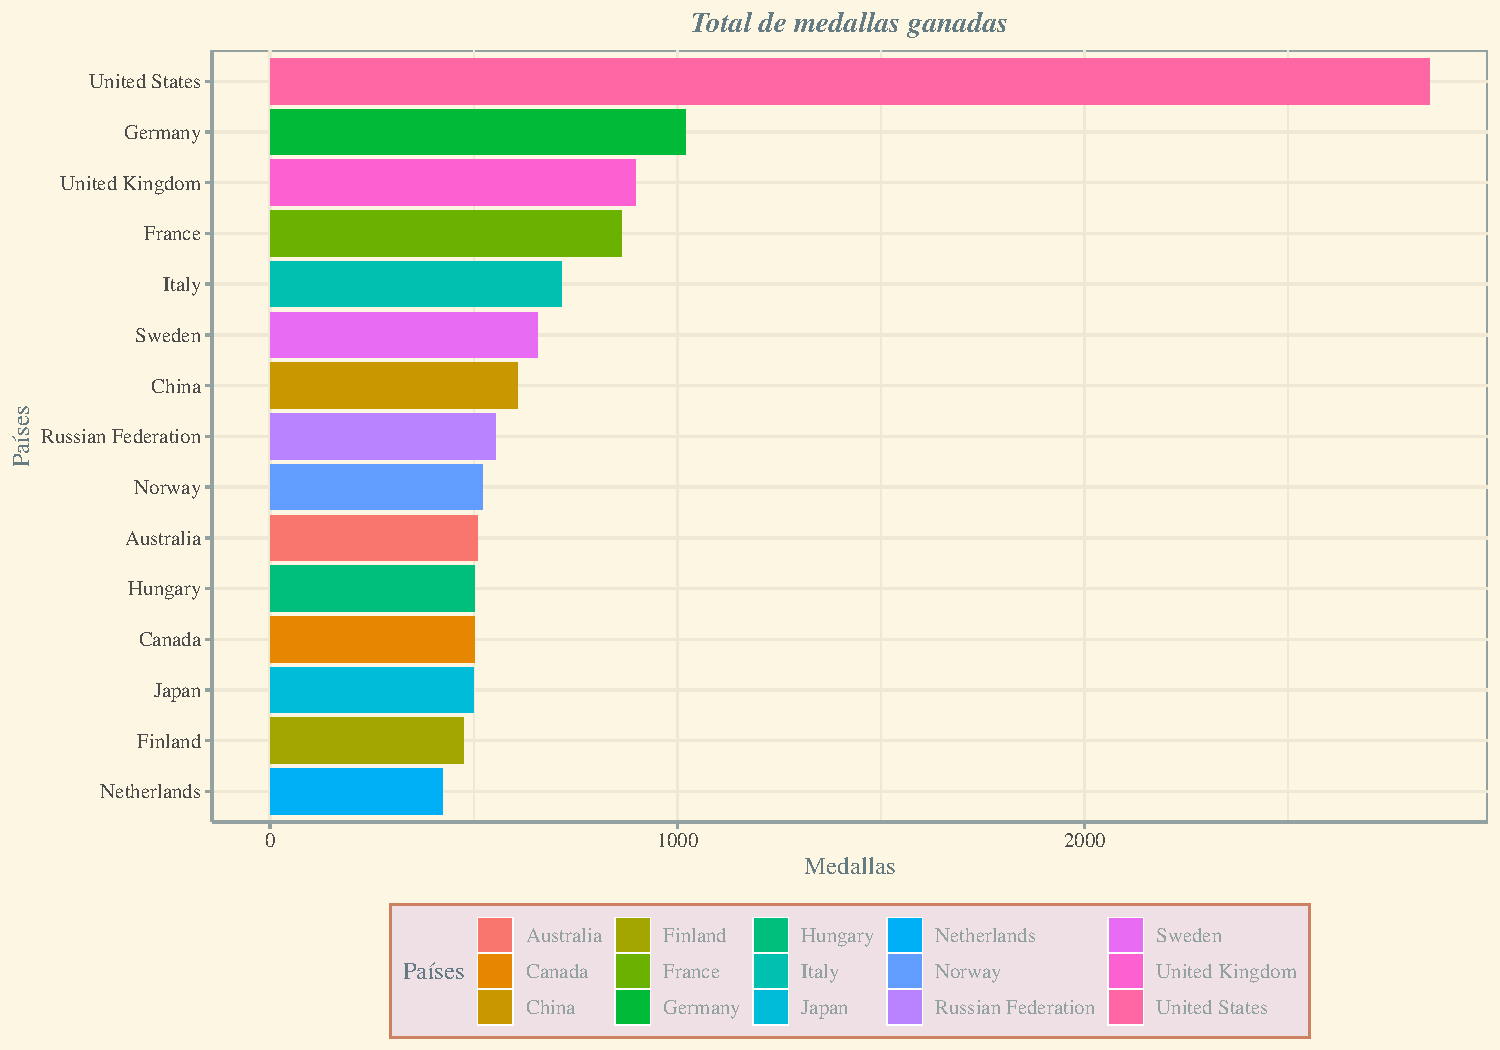
\includegraphics{Presentacion_files/figure-beamer/unnamed-chunk-9-1.pdf}
\end{frame}

\begin{frame}{Medallas y PIB}
\protect\hypertarget{medallas-y-pib-1}{}
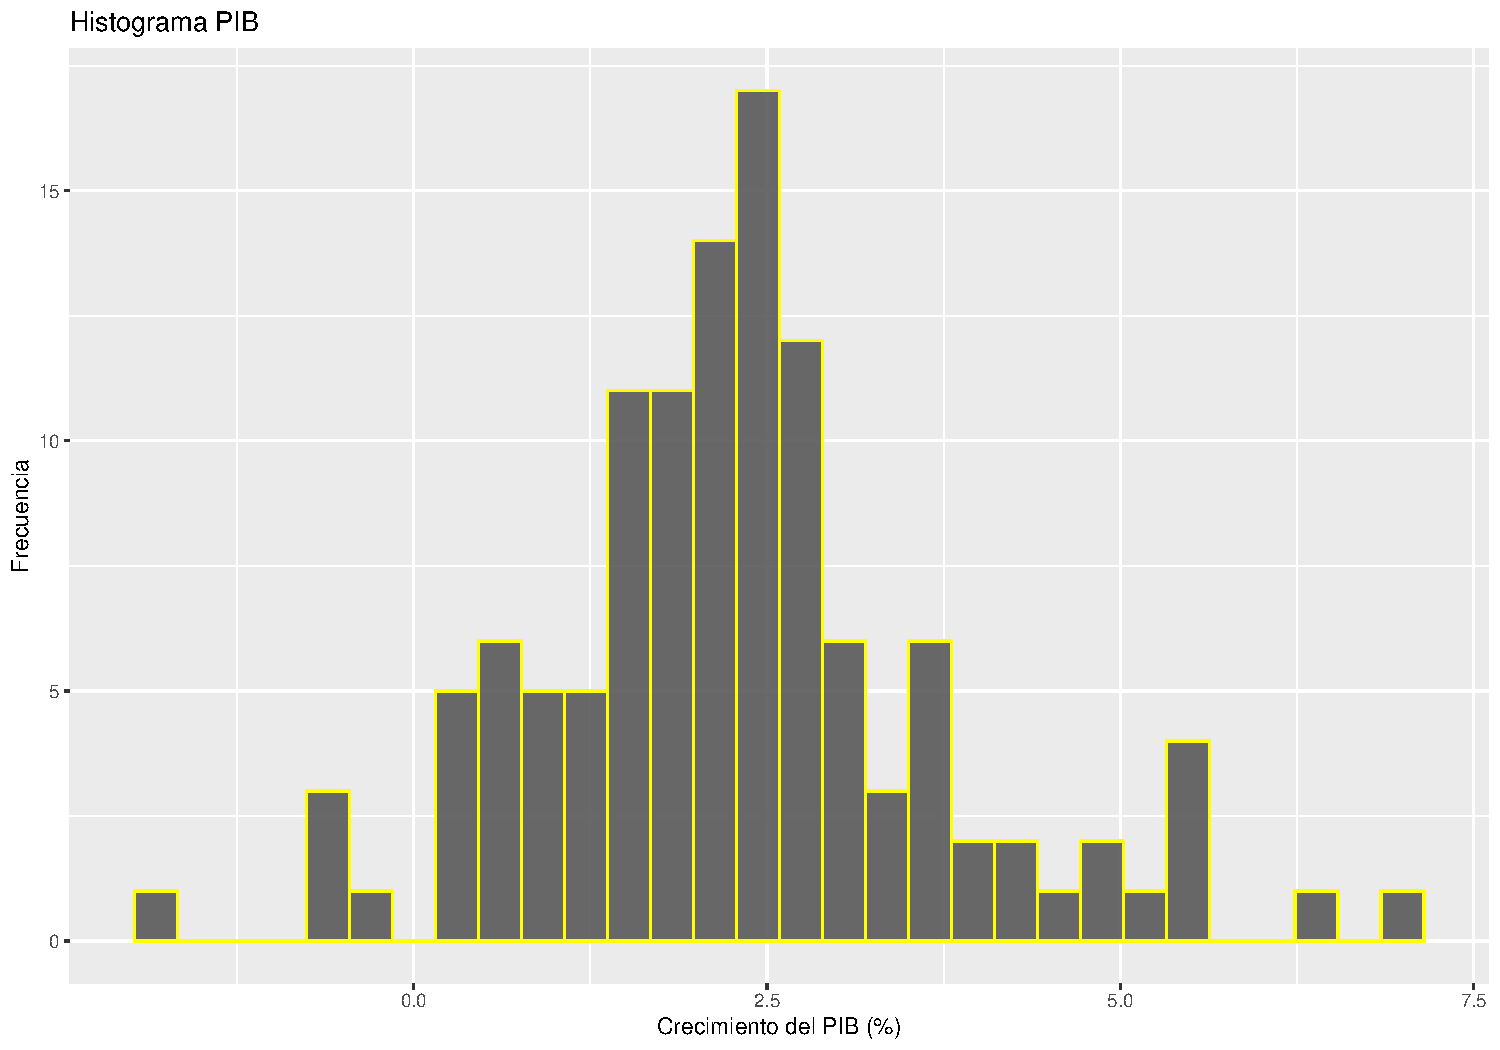
\includegraphics{Presentacion_files/figure-beamer/unnamed-chunk-10-1.pdf}
\end{frame}

\begin{frame}{Medallas y PIB}
\protect\hypertarget{medallas-y-pib-2}{}
Al analizar los diagramas de dispersión, se observa que la gran mayoría
de pares ordenados presentan correlaciones negativas entre sí, a
excepción de la relación entre la inflación y el desempleo. Se encuentra
además que la matriz de correlación expone 3 ejemplares significativos.
La primera es el desempleo y la población, la cual llega a ser
significativa a al 5\%, y es de carácter negativa. La segunda es la
relación entre el desempleo y el PIB, la cual es significativa al 10\% e
inversa. La tercera es la relación entre la inflación y el PIB, la cual
es significativa al 10\% y presenta una relación inversa entre sí.
Finalmente, se encuentra que la relación entre la inflación y el
desempleo es de carácter positiva, por lo que se establece que mayores
niveles de inflación están asociados con mayores niveles de desempleo,
tal y como afirma la teoría económica al describir el postulado de Curva
de Phillips.
\end{frame}

\begin{frame}{Correlaciones}
\protect\hypertarget{correlaciones}{}
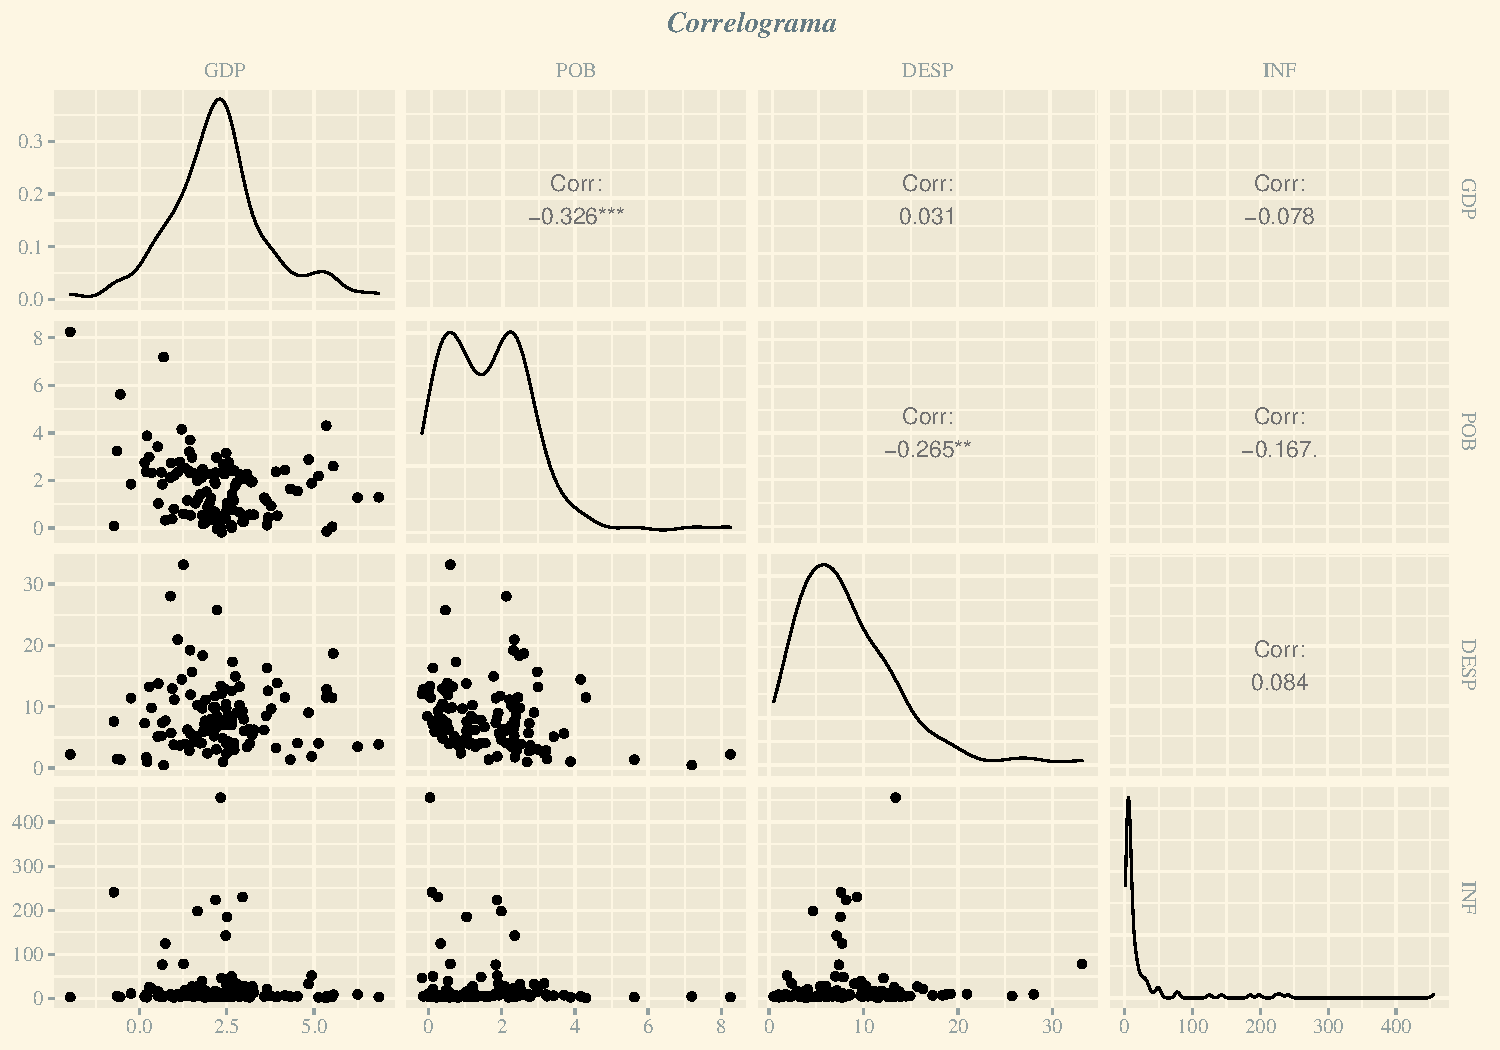
\includegraphics{Presentacion_files/figure-beamer/unnamed-chunk-11-1.pdf}
\end{frame}

\begin{frame}{Dispersión de los datos}
\protect\hypertarget{dispersiuxf3n-de-los-datos}{}
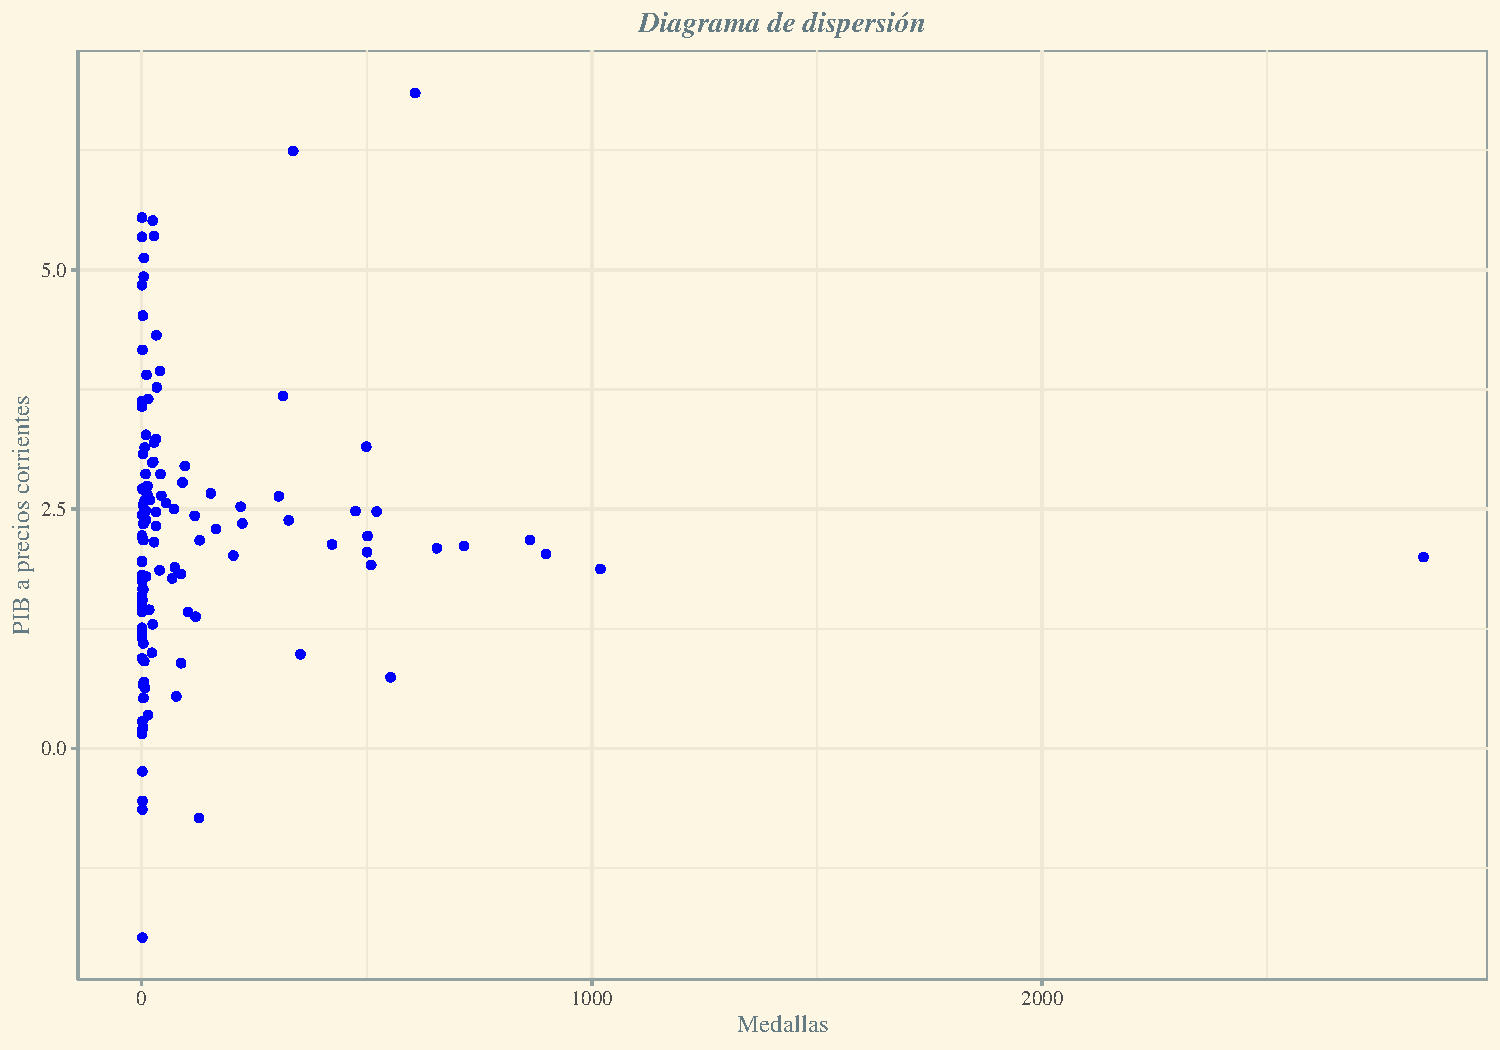
\includegraphics{Presentacion_files/figure-beamer/unnamed-chunk-12-1.pdf}
\end{frame}

\begin{frame}{Dispersión de los datos}
\protect\hypertarget{dispersiuxf3n-de-los-datos-1}{}
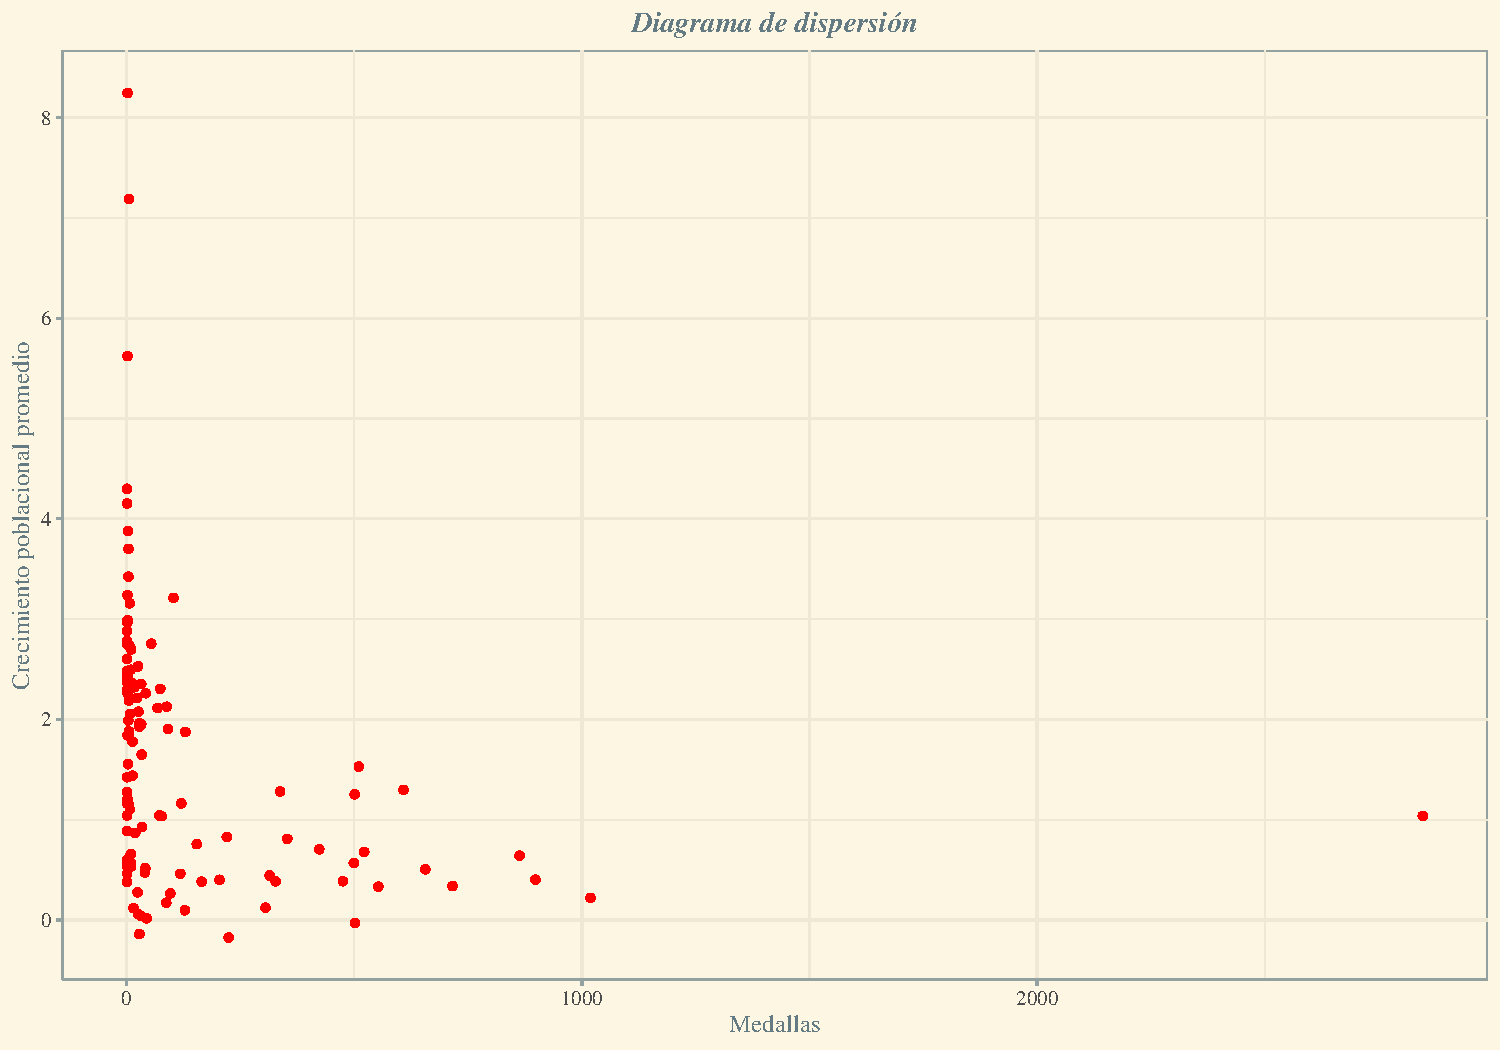
\includegraphics{Presentacion_files/figure-beamer/unnamed-chunk-13-1.pdf}
\end{frame}

\begin{frame}{Dispersión de los datos}
\protect\hypertarget{dispersiuxf3n-de-los-datos-2}{}
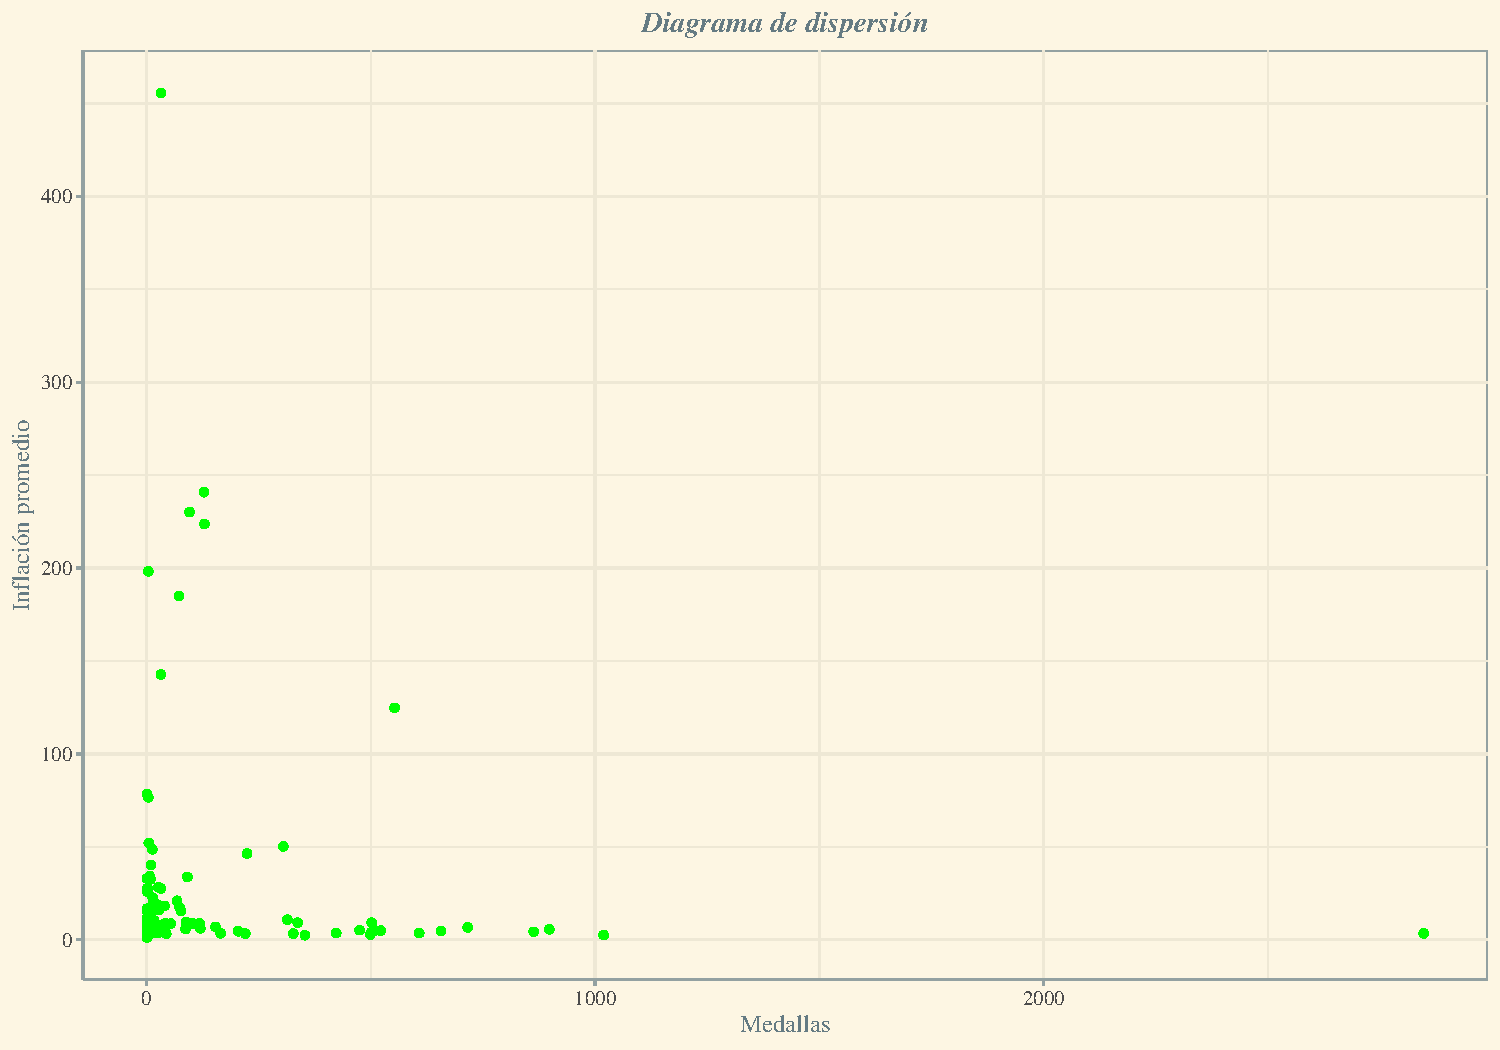
\includegraphics{Presentacion_files/figure-beamer/unnamed-chunk-14-1.pdf}
\end{frame}

\begin{frame}{Dispersión de los datos}
\protect\hypertarget{dispersiuxf3n-de-los-datos-3}{}
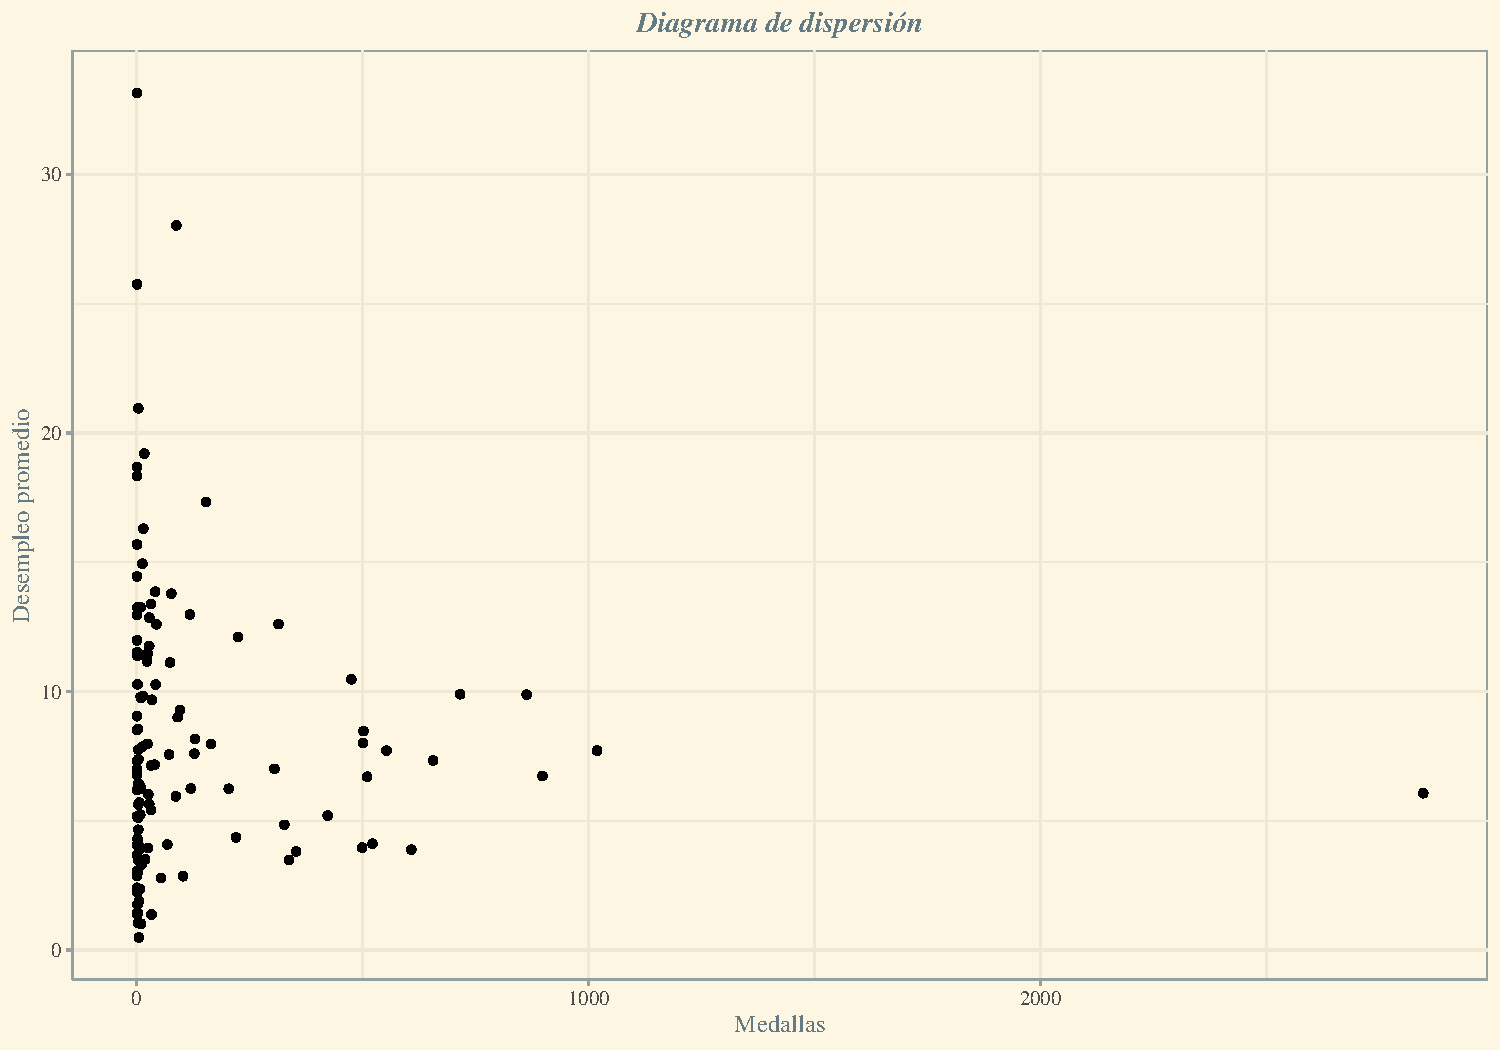
\includegraphics{Presentacion_files/figure-beamer/unnamed-chunk-15-1.pdf}
\end{frame}

\begin{frame}{Análisis preliminar}
\protect\hypertarget{anuxe1lisis-preliminar}{}
Al haber analizado las estadísticas descriptas presentadas en los puntos
anteriores, se logra observar sin lugar a duda que Estados Unidos es el
país que mayor número de medallas (entre ellas; oro, plata y bronce) ha
sumado a lo largo de la historia. Esto podría ser explicado parcialmente
por el tamaño de la población, dado que es uno de los países
participantes con mayor número de habitantes. Con respecto al análisis
agregado junto con los demás países, se encuentra que la media de
medallas ganadas por país desde 1950 hasta la actualidad corresponde a
132, sin embargo, este valor es bastante sensibles ante valores
atípicos, como lo indica la participación de Estados Unidos en los
juegos internacionales.

En cuanto al PIB corriente expresado en miles de millones de dólares, se
evidencia que la media corresponde a 7829mm de dólares norteamericanos,
además, el grado de variabilidad es bastante alto debido a que el nivel
mínimo de PIB corresponde a 159mm de dólares norteamericanos, y el
máximo a 40313mm. Al haber observado el histograma de la variable
anterior, se encuentra que la gran mayoría de los datos están
concentrados entre el mínimo y el promedio, lo cual deja en evidencia
que gran parte de los países participantes poseen bajos niveles de PIB.
Además, la distribución de la variable de acuerdo con el histograma
llega a presentar asimetría positiva, o hacia la derecha, lo cual
establece que hay diversos niveles de producto al interior las naciones
partícipes de los juegos olímpicos, donde pocos países poseen ingresos
muy altos, y la gran mayoría posee ingresos relativamente bajos. Por
otro lado, se descarta que el comportamiento de la variable se comporte
normal, debido a la asimetría positiva.

De acuerdo con los diagramas de dispersión presentados en las tablas
cruzadas, se logra establecer que todas las distribuciones presentan
asimetría positiva, de manera que se rechaza parcialmente el hecho de
que alguna variable logre presentar un comportamiento normal. Asimismo,
algunos de los cruces presentan mayor cohesión entre las observaciones,
por lo que la variabilidad de los datos es más baja para aquellas
gráficas cuyas observaciones estén más juntas. Finalmente, al haber
analizado el diagrama de dispersión de la variable dependiente e
independiente, se establece que se logra gestar una relación positiva,
donde mayores niveles de ingreso (PIB), podrían explicar mayor número de
medallas ganadas con el paso del tiempo.
\end{frame}

\begin{frame}[fragile]{Modelo}
\protect\hypertarget{modelo}{}
\begin{verbatim}
## 
## =======================================================================================
##                                             Dependent variable:                        
##                     -------------------------------------------------------------------
##                                   Numero de medallas olímpicas obtenidas               
##                              (1)                   (2)                    (3)          
## ---------------------------------------------------------------------------------------
## POB                      -155.205***            -89.416***             -77.074***      
##                           (47.184)               (23.302)               (21.652)       
##                                                                                        
## POB2                       11.717                                                      
##                            (7.943)                                                     
##                                                                                        
## GDP                        -23.938               -21.890                               
##                           (57.153)               (21.132)                              
##                                                                                        
## GDP2                        1.192                                                      
##                            (9.425)                                                     
##                                                                                        
## DESP                       -9.415*               -9.384*                -9.344*        
##                            (5.345)               (5.345)                (5.344)        
##                                                                                        
## INF                        -1.160                 -0.648                               
##                            (1.210)               (0.485)                               
##                                                                                        
## INF2                        0.001                                                      
##                            (0.003)                                                     
##                                                                                        
## Constant                 491.418***             431.823***             343.572***      
##                           (118.537)              (97.825)               (70.476)       
##                                                                                        
## ---------------------------------------------------------------------------------------
## Observations                 120                   120                    120          
## R2                          0.145                 0.122                  0.103         
## Adjusted R2                 0.091                 0.091                  0.087         
## Residual Std. Error  310.860 (df = 112)     310.874 (df = 115)     311.563 (df = 117)  
## F Statistic         2.709** (df = 7; 112) 3.987*** (df = 4; 115) 6.686*** (df = 2; 117)
## =======================================================================================
## Note:                                                       *p<0.1; **p<0.05; ***p<0.01
\end{verbatim}
\end{frame}

\begin{frame}{Pruebas}
\protect\hypertarget{pruebas}{}
\captionsetup[table]{labelformat=empty,skip=1pt}
\begin{longtable}{llll}
\caption*{
\large Akaike Information Criterion Test\\ 
} \\ 
\toprule
  &    &     &      \\ 
\midrule
 & Mod1 & Mod2 & Mod3 \\ 
AIC & 1727.7 & 1724.9 & 1723.5 \\ 
BIC & 1752.8 & 1741.6 & 1734.6 \\ 
\bottomrule
\end{longtable}

Definimos el tercer modelo como el mejor modelo pues es el que tiene
menos perdida de información.
\end{frame}

\begin{frame}{Conclusiones}
\protect\hypertarget{conclusiones}{}
\end{frame}

\end{document}
